     %%%%%%%%%%%%%%%%%%%%
     %                  %
     %  capitolo1.tex   %
     %                  %
     %%%%%%%%%%%%%%%%%%%%


\chapter{Basics of Euclidean QFT}
\noindent

The main success of the past century theoretical physics is the formulation of a class of theories called \emph{field theories},
which allow an elegant and beautiful description of both quantum systems (\emph{quantum field theory}) and statistical systems 
(\emph{statistical field theory}) using the same mathematical framework.

In this chapter I will expose a simple introduction to functional methods applied in field theories and, at the end, I will also mention briefly the main ideas of the Wilson's approach to renormalization theory,
without claiming to be too exhaustive.

For further details refer to one of the references in the bibliography, for example \cite{weinbergQFT}, \cite{Soldati3} or \cite{PS}

\section{Basic definitions}
In the following I will consider, for simplicity, the case of a neutral field $\phi$, but everything can be generalized to other fields with little modifications.
In a field theory all physical information is stored in correlation functions, objects which are defined as the expectation value of the product of $n$ fields operator, 
calculated at different spacetime points.
\begin{equation}
\langle 0 | \phi(x_1) \dots \phi(x_n)| 0  \rangle  =\mathcal{N}\int \mathcal{D} \phi\phi(x_1) \dots \phi(x_n) \e^{-S(\phi)}
\end{equation}
The normalization constant $\mathcal{N}$ is fixed requiring that $\langle1\rangle = 1$. 
The functional measure of integration is defined as:
\begin{equation}
\int \mathcal{D} \phi := \prod_{x \in \mathbb{R}^D}\int_{-\infty}^{+\infty} d \phi_x
\end{equation}
According to this definition, the position $x$ in the spacetime is treated as a discrete index, 
so the  functional integral can be imagined as a infinitely continuous generalization of a multiple Lebesgue integral.

An elegant way to define the correlation functions is as functional derivatives of a generating functional, defined in the following way:
\begin{equation}
 Z[J]  = \int \mathcal{D} \phi \e^{-S[\phi] + \langle J|\phi\rangle}
\end{equation}
here I have used the generalized dot product notation:
$$\langle J|\phi \rangle = \int d^D x J(x) \phi(y) = \int \frac{d^Dq}{(2\pi)^D} J(-q) \phi(q)$$
So we have the following expression for the $n$-point correlation function:
\begin{equation}
 \langle\phi(x_1)\dots \phi(x_n)\rangle = \frac{1}{Z[0]} \left.\left(\frac{\delta^nZ[J]}{\delta J(x_1)\dots \delta J(x_n)}\right)\right|_{J = 0}
\end{equation}
This formulation of field theories has the implication that if the partition function can be computed exactly, every correlation function can be derived from it, so the theory can be considered solved.

From the generating functional $Z$ we can define the \emph{Schwinger functional} that is, roughly speaking, a more efficient way to store the physical information:
$$W[J] =  \ln Z[J]$$% = \frac{i}{2}\int dx\int dy J(x) D_F(x - y)J(y)$$
Differentiating the Schwinger functional with respect to the external source, the connected correlation functions are obtained:
\begin{equation}\label{greenconnessa}
\left.\frac{\delta^nW[J]}{\delta J(x_1)\dots \delta J(x_n)}\right|_{J = 0} = \langle\phi(x_1)\dots \phi(x_n)\rangle_c
\end{equation}
Differentiating twice, we obtain the $2$-point connected correlation function, also called \emph{exact propagator}:
\begin{equation}\label{greenconnessa}
\left.\frac{\delta^2W[J]}{\delta J(x_1)\delta J(x_2)}\right|_{J = 0} = \langle\phi(x_1)\phi(x_2)\rangle - \langle\phi(x_1)\rangle\langle\phi(x_2)\rangle = G(x_1 - x_2)
\end{equation}
From the Schwinger functional we can also define the so called \emph{classical field}:
\begin{equation}\label{campoclassico}
 \phi_c (x) := \langle\phi(x)\rangle = \frac{\delta W[J]}{\delta J(x)}
\end{equation}
that is the normalized vacuum expectation value of the  field operator $\phi(x)$. Note that in the limit of a vanishing external source we have:
\begin{equation}\label{phiJzeri}
 \phi_c(x)|_{J=0} = \frac{\langle0|\phi(x)|0\rangle}{\langle0|0\rangle} = const
\end{equation}
(because of translational invariance). So if we exclude the possibility to have spontaneous symmetry breaking in our model, that constant must be equal to zero. 
So $\phi_c(x) =0$ if $J(x) = 0$ and \emph{vice versa}.
Now we can define the \emph{effective action} $\Gamma[\phi_c]$ as the Legedre functional transformation of the Schwinger functional:
\begin{equation}\label{lagamma}
 \Gamma [\phi_c] := \sup_J \Big(\langle J \phi_c  \rangle - W[J]\Big)
\end{equation}
We note that the effective action, being a Legendre transform, has the property to be convex:
\begin{equation}
\frac{\delta^2 \Gamma}{\delta\phi \delta\phi} \geq 0
\end{equation}
that means, in the language of operators, that the second functional derivative of the effective action has positive semidefinite eigenvalues.
\section{Proper Vertices}
Differentiating the effective action with respect to the classical field and evaluating the result for a vanishing classical field, we obtain
the so called \emph{proper vertices} of the theory:
\begin{equation}
\Gamma^{(n)} (x_1 \dots x_n) = \frac{\delta^{(n)}\Gamma[\phi_c]}{\delta\phi_c(x_1) \dots \delta \phi_c (x_n)}
\end{equation}
In this way, the effective action can be expressed as an expansion in powers of the classical fields, the proper vertices being the coefficients of the expansion:
\begin{equation}
\Gamma[\phi_c] = \sum_{n = 0}^\infty \frac{1}{n!}\prod_{j = 1}^{n}\int d^D x \phi_c(x_j)\Gamma^{(n)}(x_1, \dots, x_n)
\end{equation}
These functions are translation invariant, so their expressions in momentum space read:
\begin{equation*}
 \Gamma^{(n)}(x_1, \dots, x_n) = \int\frac{d^Dp_1}{(2\pi)^D}\e^{-ip_1x_1} \dots \int\frac{d^Dp_n}{(2\pi)^D} \e^{-ip_nx_n}\Gamma^{(n)}(p_1, \dots, p_n)(2\pi)^D\delta(p_1 + \dots p_n )
\end{equation*}

Let's perform the calculation of some of the firsts of them. The first term of the expansion is :
\begin{equation}
 \Gamma^{(0)}  \equiv \Gamma[0] =  0
\end{equation}
In order to obtain $\Gamma^{(1)}$, we have to differentiate once equation \eqref{lagamma} obtaining:
\begin{equation}
 \Gamma^{(1)}[\phi_c] =\left[ J(x) + \int d^Dy \frac{\delta J(y)}{\delta \phi_c (x)}\phi_c(y) -  \int d^Dy \frac{\delta J(y)}{\delta \phi_c (x)}\frac{\delta W[J]}{\delta J(y)} \right]_{\phi_c = 0}
\end{equation}
\begin{equation}
= \left.\frac{\delta \Gamma[\phi_c]}{\delta \phi_c} \right|_{\phi_c = 0} = J(x) 
\end{equation}

For the $2$-point proper vertex we start from the definition:
\begin{equation}
 \Gamma^{(2)}(x - y) = \left.\frac{\delta^2\Gamma[\phi_c]}{\delta\phi_c(x)\delta\phi_c(y)}\right|_{\phi_c=0} = \int\frac{d^Dp}{(2\pi)^D}\Gamma^{(2)}(p) \e^{-ip(x-y)}
\end{equation}
Recalling the definition of the classical field $\phi_c$ \eqref{campoclassico}, the following relations hold true:
\begin{equation}
 \frac{\delta^2W[J]}{\delta J(x) \delta J(y)} =  \frac{\delta \phi_c(x)}{\delta J(y)} = \left[\frac{\delta J(y)}{\delta \phi_c(x)}\right]^{-1} = \left[\frac{\delta^2\Gamma[\phi_c]}{\delta\phi_c(x)\delta\phi_c(y)}\right]^{-1}
\end{equation}
From this we obtain the following important relation:
\begin{equation}\label{importanterelazione}
 \int d^Dy \frac{\delta^2W[J]}{\delta J(x) \delta J(y)}\frac{\delta^{(2)}\Gamma(\phi_c)}{\delta\phi_c(y)\delta\phi_c(z)} = \delta(x - z)
\end{equation}
From eq.\eqref{importanterelazione}, after setting both the external source and the classical field equal to zero
and recalling the definition of the propagator \eqref{greenconnessa} we obtain:
\begin{equation}
\int d^Dy G(x - y) \Gamma^{(2)} ( y - z) = \delta(x - z)
\end{equation}
Or, in momentum space:
\begin{equation}
  G(p)\Gamma^{(2)}(p) = 1
\end{equation}
To calculate the $3$-points proper vertex, equation \eqref{importanterelazione} has to be differentiated with respect to the external source.
The result is:
\begin{equation}\label{soldati3punti}
 \frac{\delta^3W}{\delta J_x \delta J_y \delta J_v}*\frac{\delta^2\Gamma}{\delta\phi^y_c\delta\phi^z_c} + \frac{\delta^2W}{\delta J_x \delta J_y}*\frac{\delta^2W}{\delta J_v \delta J_w}*\frac{\delta^3\Gamma}{\delta\phi^w_c\delta\phi^y_c\delta\phi^z_c} = 0
\end{equation}
where I use the discrete index type notation, and the convolution product over repeated index is understood.
In order to obtain the second term of the previous expression, the following relation has to be used:
\begin{equation}
\frac{\delta}{\delta J(v)}\left(\frac{\Gamma^{(2)}[\phi_c]}{\delta\phi_c(x)\delta\phi_c(y)}\right) = \int dw \frac{\delta^3\Gamma[\phi_c]}{\delta\phi_c(x)\delta\phi_c(y)\delta\phi_c(w)}\cdot\frac{\delta\phi_c(w)}{\delta J(v)}= 
\end{equation}
\begin{equation*}
 =  \int dw \frac{\delta^3\Gamma[\phi_c]}{\delta\phi_c(x)\delta\phi_c(y)\delta\phi_c(w)}\cdot\frac{\delta^2W[J]}{\delta J(v)\delta J(w)}
\end{equation*}
Setting the classical field equal to zero and recalling the fact that the $n$-point connected correlation functions are defined as the $n^{th}$ order functional derivatives of the 
Schwinger functional with respect to the source we can rewrite equation \eqref{soldati3punti} in the following way:
\begin{equation}
 G^{(3)}_{xyv}*\Gamma^{(2)}_{yz} + G^{(2)}_{xy} *G^{(2)}_{vw}*\Gamma^{(3)}_{wyz} = 0
\end{equation}
And:
\begin{equation}
 \Gamma^{(3)}_{wyz} = -G^{(3)}_{xyv}*\Gamma^{(2)}_{yz} *\Gamma^{(2)}_{xy} *\Gamma^{(2)}_{vw} = - G^{(3)}_{xyv}*\left(G^{(2)}_{yz}\right)^{-1} *\left(G^{(2)}_{xy}\right)^{-1} *\left(G^{(2)}_{vw}\right)^{-1}
\end{equation}
So, we come to the conclusion that the $3$-point proper vertex is, exept for the minus sign, nothing but the connected $3$-point Green's function in which all the external propagator have been 
amputated.

So we have deduced that the $3$-point proper vertex is, exept for the minus sign, the connected $3$-point green function in which the external full propagators have been amputated. 

A similar reasoning can be made, by induction, for the generic $n^{th}$ order derivative of $\Gamma$, 
obtaining the result that the effective action is the generating functional of all the $n$-point proper vertices.

\begin{table}
  \begin{center}
    \begin{small}
      \begin{tabular}{|c|c|c|}

\hline
 \textbf{QFT quantity}& \textbf{Symbol} & \textbf{SM analogous} \\
\hline
Generating functional& $Z$  & Canonical partition function \\
\hline
Generator of the connected c.f. & $W$  &  $-\beta \cdot$ Helmoltz free energy\\
\hline
External source & $J$ & generalized external parameter \\
\hline
Classical field & $\phi_c$ & generalized external force\\
\hline
Effective action & $\Gamma$ & Gibbs free enthalpy\\
\hline
Classical action & $S$ & dimensionless Hamiltonian ($\beta{\mathcal{H}}$)\\
\hline
      \end{tabular}
    \end{small}
  \end{center}
\caption{The Euclidean QFT and the statistical mechanics share the same general mathematical structure. 
That means that we can eventually obtain the one from the other simply taking into account the correspondances illustrated in this table. 
I recall the definition of the thermodynamic $\beta$ as the reciprocal of the absolute temperature, $\beta = (k_B T)^{-1}$, where $k_B$ is the Boltzmann constant.}
\label{tab:QFTeSM}
\end{table}

\section{Effective potential}
The definition of the effective action $\Gamma(\phi_c)$ leads to the concept of the effective potential $U$,
which reveals to be an useful tool in the study of the long range physics or in the understanding of the phenomenon
of the spontaneous symmetry breaking. 

By definition, $U(\bar{\phi})$ is simply the effective action calculated in a constant
classical field configuration, $\phi_c = \bar{\phi}$:
\begin{equation}
U(\bar{\phi}) = \sum_{n = 2}^{\infty}\frac{\bar{\phi}^n}{n!}   \Gamma^{(n)}(0, \dots, 0)
\end{equation}
Thus we have, in coordinate space:
\begin{equation}
\Gamma[\bar{\phi}] = \sum_{n = 2}^{\infty}\frac{\bar{\phi}^n}{n!}\int dx_1 \dots \int dx_n \Gamma^{(n)}(x_1, \dots, x_n)
\end{equation}
So, in momentum space:
\begin{equation}
 \Gamma[\phi] = \sum_{n = 2}^{\infty}\frac{\bar{\phi}^n}{n!} \prod_{j = 1}^n \int dx_j \int\frac{d^D k_j}{(2\pi)^D} \e^{-ik_jx_j} (2\pi)^D \delta\left(\sum_{i=m}^n k_m\right)\Gamma^{(n)}(k_1, \dots, k_n) =
\end{equation}
$$= \sum_{n = 2}^{\infty}\frac{\bar{\phi}^n}{n!} \int d^D k_1 \delta(k_1) \dots \int d^D k_n \delta(k_n)  (2\pi)^D \delta\left(\sum_{i=1}^n k_i\right)\Gamma^{(n)}(k_1, \dots, k_n) =$$
$$= \sum_{n = 2}^{\infty}\frac{\bar{\phi}^n}{n!}   (2\pi)^D \delta\left(0\right)\Gamma^{(n)}(0, \dots, 0) =$$
$$=(2\pi)^D \delta\left(0\right) U(\bar{\phi})$$

 
 
\section{Wilson's approach to renormaliztion}
The \emph{Wilson's renormalization group} was formulated by Kenneth Wilson and coautors in the $70$s in a series of  pioneering papers (\cite{wilson1}\cite{wilson2}\cite{wilson3})
and nowadays it is the essence of modern renormalization theory. 

Here I will recall the basic concepts of it, because it will be the basis for the nonperturbative Wetterich's formulation of
the renormalization group, on which this work is based.

\subsection{Kadanoff's block spin}
The basic idea of renormalization is due to Leo Kadanoff \cite{Kadanoff} who, before the Wilson's formal and mathematically rigorous formulation of the renormalization group techniques,
proposed a heuristic physical picture which provided the conceptual basis for the scaling behavior. 

That was the Kadanoff's transformation, which allows to eliminate the small wavelength degree of fredoomon from the physical description of 
a spin chain system dividing it into blocks and doing a local average in order to obtain an ``effective spin'' for each block (this step is also called \emph{decimation}) and
the system is rescaled.

In the following I will give a sketch of the procedure. The partition function reads:
\begin{equation}
 Z = \sum_{S_i} \e^{-\beta\mathcal{H}[S_i]}
\end{equation}
Defining $a$ the lattice size, we divide it into blocks of size $\alpha^D$, where $D$ is the dimension of the space (so, in our example, $D=2$)
and $\alpha$ is the \emph{spatial rescaling factor}. Then one averages out the spins in each block, obtaining an
\emph{effective spin} for each block. 
So we can compare the new system with the previous one performing a rescaling $\alpha a \to a$.
After this operation, we have a rescaled system described by the effective partition function:
\begin{equation}
 Z = \sum_{S_A} \e^{-\beta\mathcal{H}_{eff}[S_A]} = \sum_{S_i} \sum_{S_A}\prod_A\delta\left(S_A - \alpha^{-D}\sum_{i \in A}{S_i} \right)\e^{-\beta\mathcal{H}[S_i]}
\end{equation}
but, because of the relations:
$$\sum_{S_A}\prod_A\delta\left(S_A - \alpha^{-D}\sum_{i \in A}{S_i} \right) = 1$$
we have that the partition function is left unchanged by the scaling transformation:
\begin{equation}
 Z = \sum_{S_A} \e^{-\beta\mathcal{H}_{eff}[S_A]} = \sum_{S_i}\e^{-\beta\mathcal{H}[S_i]}
\end{equation}
and the new effective Hamiltonian describes the same long range physics of the previous one.

The idea is to iterate this procedure an infinite number of times, obtaining after each step a new effective Hamiltonian 
at larger scales:
$$\mathcal{H}^{0}\to\mathcal{H}^{1}\to\mathcal{H}^{2}\to\mathcal{H}^{3}\to\mathcal{H}^{4}\to\dots \to\mathcal{H}^{N}\to\dots $$
In an Ising model one of the central observable the correlation lenght $\xi$, that  is defined in terms  of the two point correlation function of spins.
If we choose two point $x$ and $y$ on the lattice, one can write the correlation functions in  the following way:
\begin{equation}
 G(x-y) \approx \e^{-\frac{|x-y|}{\xi}}
\end{equation}
Obviously the correlation lenght change with the scale. After every step, it is reduced by a factor $\alpha$:
$$\xi \to \frac{\xi}{\alpha}$$
If this lenght (and all the other observable of the system) is left unchanged by the rescaling transformation, 
we have what is called a \emph{fixed point}. This can happen in two different situations:
\begin{equation}
\left\{
\begin{array}{l}
\xi \to \infty \ \ \ \ \ \  \ \ \ \ \text{critical fixed point}\\
\xi \to 0 \ \ \ \ \ \  \ \ \ \ \text{trivial (or Gaussian) fixed point}
\end{array}
\right.
\end{equation}
So this technique is suitable to study the behavior of the system near a phase transition.
\begin{figure}
\begin{center}
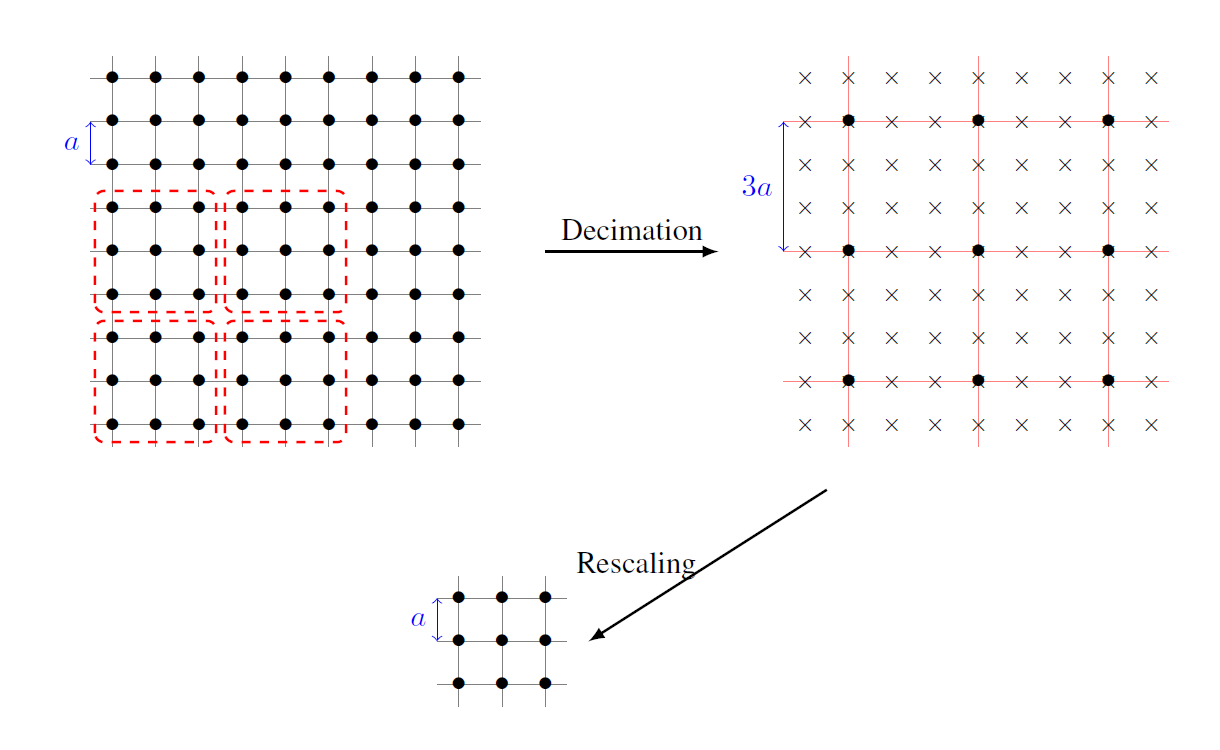
\includegraphics[scale=0.38]{Immagini/kadanoff.png}
\caption{An illustration of the Kadanoff procedure applied on a bidimensional ($D=2$) Ising system with size $a$.
The initial lattice is divided into blocks of size $9$ (so $\alpha = 3$), an effective spin for each block is computated
and an effective spin $S_A$ is obtained. To recover the initial lattice the rescaling $3a\to a$ is performed. \cite{karim}}
\label{fig:ising}
\end{center}
\end{figure}

\subsection{Wilson Momentum shell integration}
The idea of the Kadanoff s block spin can be extended to a system whose degree of freedom are encoded in a field $\phi(x)$,
which we assume to be a continuous function of space and time.

In order to obtain an effective description of the physics of the system in the low momentum (\emph{i.e.}, long distance) regime,
we have to separate the contribution of the modes with momentum higher and lower of a given coarse graining scale $k$:
\begin{equation}
\phi(q) = \phi_< (q) +\phi_> (q)
\end{equation}
The low momentum modes $\phi_<$ and the high momentum ones $\phi_>$ are defined in the following way:
\begin{equation}
 \phi_< (q) = \theta(k-|q|)\phi(q)
\end{equation}
\begin{equation}
\phi_> (q)= \theta(k-|q|)\phi(q)
\end{equation}
In view of that, and recalling the definition of the generating functional in presence of a given ultraviolet cutoff $\Lambda$,
(that is the analogous of the initial lattice space in Kadanoff's model so, in a certain sense, we can say  $\Lambda = a^{-1}$) we have:
\begin{equation}
  Z = \int \prod_{|q| \leq \Lambda}d\phi_q\e^{-S_\Lambda[\phi]} 
\end{equation}
we can write:
\begin{equation}
   Z = \int \prod_{|q| \leq k}\prod_{k\leq |q| \leq \Lambda}d\phi_q\e^{-S_\Lambda[\phi]} = \int \prod_{|q| \leq k }d\phi_q\e^{-S_k[\phi]}=   \int \mathcal{D} \phi_< \e^{-S_k[\phi_<]}
\end{equation}
where the running action (also called the \emph{Wilsonian average action}) is defined in the following way:
\begin{equation}
 \e^{-S_k[\phi_<]} = : \int  \prod_{k\leq |q| \leq \Lambda}d\phi_q\e^{-S_\Lambda[\phi]} =   \int \mathcal{D} \phi_> \e^{-S[\phi]}
\end{equation}
In this way we have arrived to a complicated functional integral equation, describing the dependence of the Wilsonian equation
on the scale parameter $k$. 

When $k=\Lambda$ the running action reduces to the classical bare action, which describes the 
the physics of the system in the ultraviolet limit, conversely when $k \to 0$, all the fluctuations are included in the description
of the model, giving us the complete microscopic quantum field theory.

In the intermediate region we may interpret $S_k$ as an effective action describing under certain approximation the physics at the scale 
$k$. A reason to believe that is the fact that, by definition, only modes with $|q| \approx k$ are active on the scale $\sim k^{-1}$.

When this ideas are implemented, one obtains that the exact evolution equation for $S_k$ depends on a certain cutoff function $K_k(q)$.
The equation describing the evolution of $S_k$ has been derived for the first time in \cite{wilson2} for a smooth cutoff function and
in \cite{cinquantotto} for a sharp cutoff.

The most used version of this evolution equation, with a non specified cutoff function, has been derived by J. Polchinski in  \cite{Polchinski} and reads:
\begin{equation}\label{wilson}
 \partial_kS_k = \frac{1}{2} \int \frac{d^Dq}{(2\pi)^D}\partial_kK_k(q)\left(\frac{\delta^2S_k}{\delta \phi_<(q)\delta \phi_<(-q)}- \frac{\delta S_k}{\delta \phi_<(q)}\frac{\delta S_k}{\delta \phi_<(-q)}\right)
\end{equation}
This equation encodes all the perturbative and nonperturbative effects of the model under consideration, given the bare action $S_\Lambda$.
However some problematic aspects have to be considered in order to use equation \eqref{wilson} for practical purpose. For example, if we want to compute any observable out of the running action $S_k$, we still have to compute the partition function, and that implies a functional integration over the low momenta modes $\phi_<$.

Another problem that arise is the non locality, because in eq.\eqref{wilson} modes of different momenta are coupled together. 


Because of those difficulties related to the Wilson procedure, alternative formulations seem to be desirable.

An alternative approach to functional renormalization that has been developed in recent years 
is due to Wetterich, and  it is focalized on a scale
dependent effective action $\Gamma$, rather than on a scale dependent action.

In this thesis I have used this approach, that will be extensively discussed in the following chapter.



\subsubsection{Fixed Points}
The behavior of an interacting field theory is characterized by a set of scale dependent couplings $g_{i,k}$, that I will define in the following way:
$$ \Gamma_k\left[\phi\right]=\sum_i g_{i,k}\mathcal{O}_{i}\left[\phi\right]$$
Where the $\mathcal{O}_{i,k}$ is an appropriate set of operator that span the space to which the scale dependent effective action belongs to 
and that are compatible with the symmetries of the system. For simplicity I have chosen a basis of operator that does not flows, 
so $\mathcal{O}_i$ is independent of $k$.
Taking the $t$-derivative of the effective action:
$$ \dot{\Gamma}_k\left[\phi\right]=\sum_i \beta_i \mathcal{O}_i\left[\phi\right]$$
we can define the \emph{beta functions}. By definition, the beta function $\beta_i$ associated to the coupling $g_i$ is simply its 
$t$ derivative and it depends on the scale and on the coupling itself.

A fixed point is defined as a point where all the beta functions vanishes:
\begin{equation}
 \beta_i (g_i^*) = 0
\end{equation}
where $g_i^*$ is the $i^{th}$ coupling calculated at the fixed point.

Obviously the fixed points are scale invariant points, 
so if we take it as initial condition of the flow, our theory will remain there at every scale. 
In general a given running theory will have several fixed points or even a continuum of fixed points forming a manifold 
in the coupling space.

Each fixed point has its own \emph{basin of attraction}, which is the set of points in coupling constant space which flow inside  
 it when the effective average action flows, so we can see a fixed point as a point where flow lines start or end.

 The study of the behavior of the flow in the proximity of a given fixed point is usually done defining the \emph{stability matrix} in the following way:
\begin{equation}
\left.\mathcal{M}_{ij} \right|_{g^*}=\frac{\partial {\beta}_i}{\partial {g}_j} 
\end{equation}
This matrix can be diagonalized in order to obtain a set of eigenvalues:
\begin{equation}
 \left.\mathcal{M}_{ij}\right|_{{g}^*}=\text{diag}\left(\omega_1,\omega_2,\dots\right)
\end{equation}
A negative eigenvalue means that the fixed point is attractive in the correspondig direction, the converse is true if the eigenvalue is positive.

\subsubsection{Critical exponents}
If we are following the flow close to the fixed point along the direction $v_i$ (where I have indicated with $v_i$
the eigenvector associated to the $i^{th}$ eigenvalue) the coupling constant can be expressed as the sum of its value
at the fixed point $g_i^*$ plus a small fuctuation around this value:
\begin{equation}
 g_i = g_i^* + \delta g_i
\end{equation}
thus we can linearize the flow equation obtaining:
\begin{equation}\label{expcr}
 \delta \dot{g}_i = \left. \frac{\partial \beta_i}{\partial g_j} \right|_{g^*}\delta g_j = \left.\mathcal{M}_{ij} \right|_{g^*}\delta g_j
\end{equation}
Now we should solve the eigenvalue problem:
\begin{equation}\label{auto}
\left.\mathcal{M}_{ij} \right|_{g^*} v_j^{(a)} = \omega_a v_j^{(a)}
\end{equation}
and expand the coupling constant vector in terms of the basis given by the eigenvector of $\mathcal{M}$:
\begin{equation}\label{c}
 \delta g_i = \sum_a c_a v_i^{(a)}
\end{equation}
where the $c_a$ are some constant to be found.
Now, substituting equation \eqref{c} and \eqref {auto} into the equation \eqref{expcr}, we come to the result:
\begin{equation}
 \dot{c}_a = \lambda_a c_a
\end{equation}
that has the solution:
\begin{equation}
 c_a(t) = c_a(0) \e^{\lambda_a t} = c_a(0)\left(\frac{k}{k_0}\right)^{\lambda_a}
\end{equation}
The \emph{critical exponents}  of the model are defined as:
\begin{equation}
 v_a = -\lambda_a
\end{equation}
and, depending on their sign, the corresponding direction in coupling space is said:
\begin{enumerate}
 \item relevant, if $v_a > 0$;
 \item marginal, if $v_a = 0$;
 \item irrelevan, if $v_a <0$;
\end{enumerate}
In terms of dimensionless quantities (\emph{i.e.} dimensionless couplings) if in the UV a fixed point exist with finite values
of the couplings $g_i^*$ and if there exists a finite number of relevant directions, then the theory is said to be 
renormalizable, even if interacting (this is called \emph{asymptotic safety} \cite{weinberg}).

Yang Mills theories are special cases of asymptotic safety called \emph{asymptotic freedom}, since $g_i^* = 0$ at the fixed point.

